\section{Results}\label{sec:results}

The results come in three parts: the training period, whose numbers were frozen before the vote; the pre-registered
midterm test; and exploratory analyses carried out after the vote. Only the second part is confirmatory.

\subsection{The training period}

\paragraph{General elections are underconfident, Kalshi's primaries are not.}
Table~\ref{tab:training} reports the stretch for every group in the training data. On the general-election night of
5 November 2024, the stretch was 1.97 on Kalshi, with an interval from 1.27 to 3.77 that lies entirely above 1, and 1.83
on Polymarket, with an interval from 0.99 to no upper limit. Across all training general elections, the stretch was 1.28
on Kalshi and 1.61 on Polymarket. These general-election groups span only six or seven election days, and one of them,
5 November 2024, holds most of the contests, so resampling whole days gives very wide intervals; resampling states,
which keeps every day in, gives intervals of 0.83 to 2.62 and 0.80 to no upper limit. Kalshi's 78 primaries point the
other way: a stretch of 0.32, with 99\% of day resamples at or below 1. Polymarket's 23 primaries are close to
calibrated (0.88). Pooling everything, Kalshi's markets look overconfident (0.58, 97\% of resamples at or below 1),
because its primaries outnumber its general elections.

\begin{table}[htbp]
\centering\small\setlength{\tabcolsep}{4.5pt}
\caption{The stretch in the training period, frozen before the vote. Intervals are 95\%; ``no limit'' means enough
resamples had every favourite winning that the stretch has no upper bound. The frozen fitting routine stops at the
wrong value on a few resamples of Kalshi's election days (Section~\ref{sec:limitations}); with a corrected routine,
Kalshi's day-resampled intervals are 0.14 to 1.02 for all contests and 0.01 to 0.69 for primaries, and nothing else in
the table changes.}\label{tab:training}
\begin{tabular}{llrrrll}
\toprule
 & Group & Contests & Days & Stretch & Days resampled & States resampled \\
\midrule
Kalshi & All & 152 & 26 & 0.58 & 0.14 to 1.03 & 0.39 to 0.86 \\
 & General elections & 74 & 6 & 1.28 & $-0.77$ to no limit & 0.83 to 2.62 \\
 & Primaries & 78 & 21 & 0.32 & 0.03 to 0.70 & 0.10 to 0.58 \\
 & 5 November 2024 & 60 & 1 & 1.97 & & 1.27 to 3.77 \\
\midrule
Polymarket & All & 64 & 23 & 1.23 & 0.58 to 1.75 & 0.75 to 2.19 \\
 & General elections & 41 & 7 & 1.61 & 0.33 to no limit & 0.80 to no limit \\
 & Primaries & 23 & 17 & 0.88 & 0.40 to 1.67 & 0.40 to 1.56 \\
 & 5 November 2024 & 35 & 1 & 1.83 & & 0.99 to no limit \\
\bottomrule
\end{tabular}
\end{table}

Figure~\ref{fig:train_calibration} shows the same results as calibration charts. Contests are grouped by the
favourite's price; each dot is the share of favourites that won, and the curve is the fitted stretch. In general
elections the dots sit on or above the diagonal, and every favourite priced above 90\% won. In Kalshi's primaries, the
dots sit well below it: favourites priced between 70\% and 90\% won barely more than half the time.
Figure~\ref{fig:train_stretch} shows the stretch with both kinds of interval, and the distribution of the resampled
stretch for all contests together.

\begin{figure}[tbp]
\centering
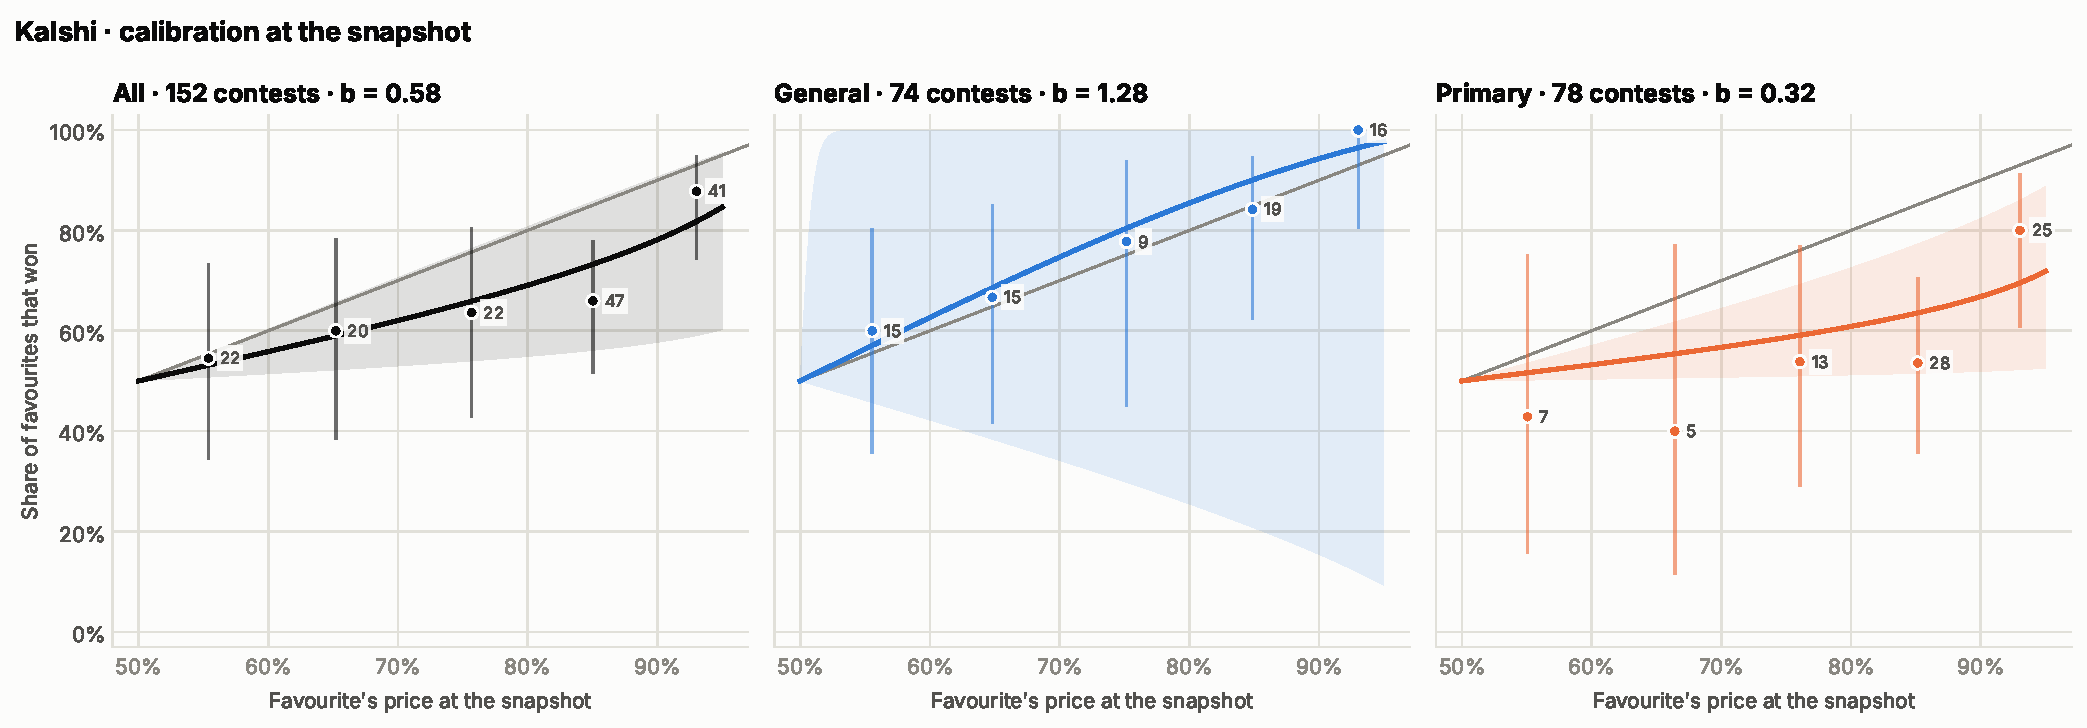
\includegraphics[width=\textwidth]{figures/fit_kalshi_calibration.pdf}\par\medskip
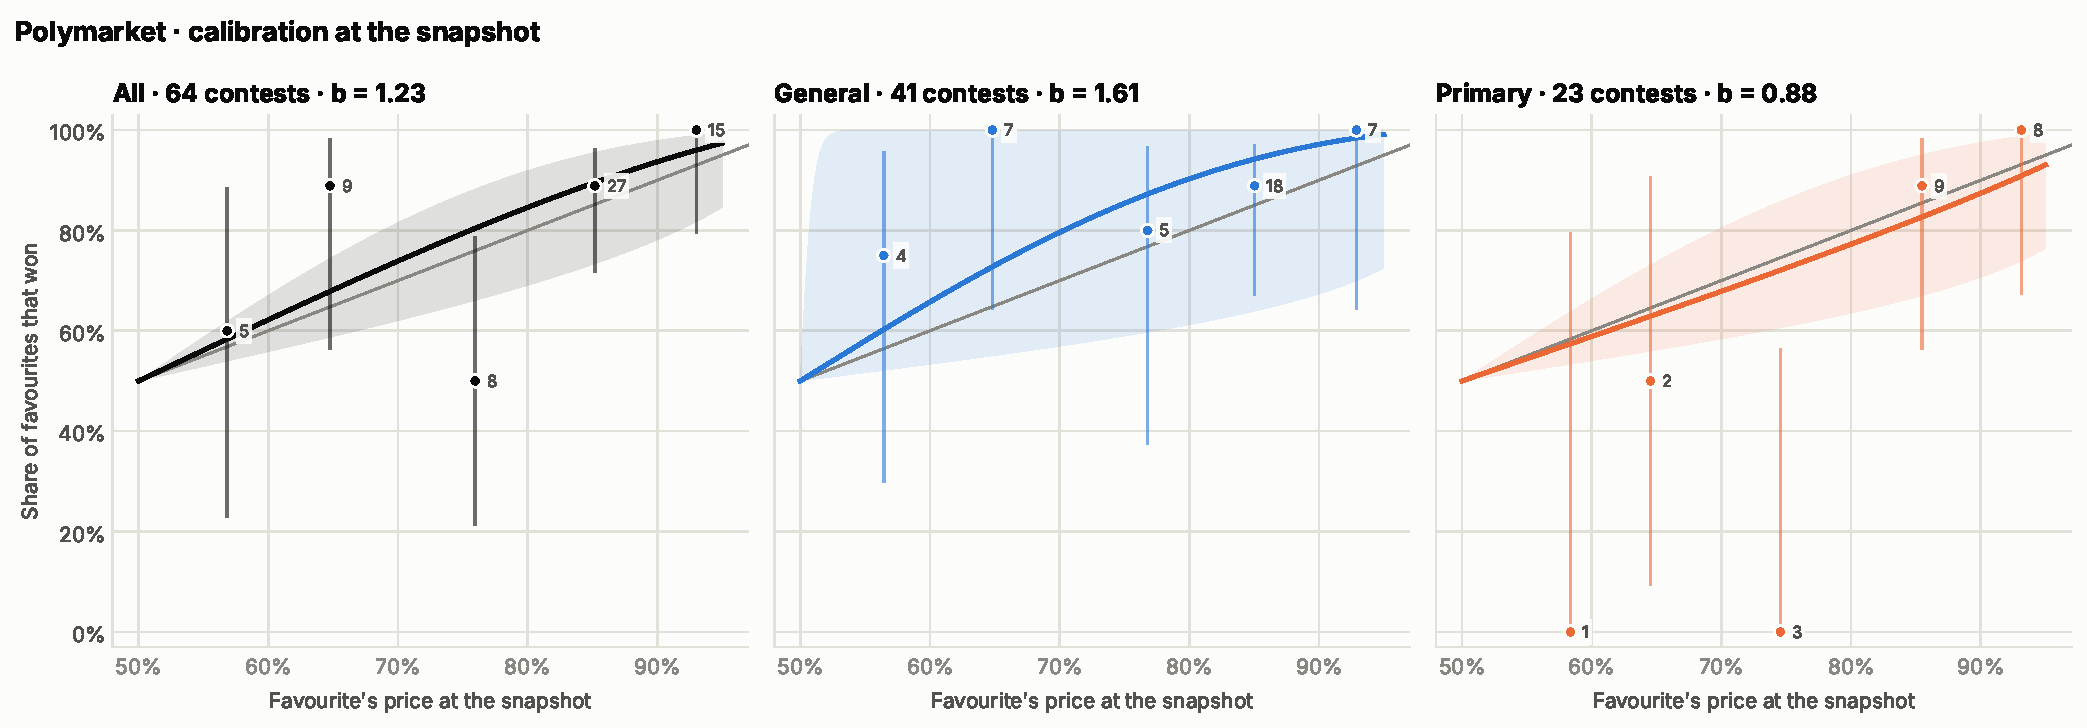
\includegraphics[width=\textwidth]{figures/fit_polymarket_calibration.pdf}
\caption{Calibration in the training period. Dots: share of favourites that won in each price group, with 95\%
intervals and the number of contests. Curve: the fitted stretch, with the range covered by its interval shaded. Grey
diagonal: a calibrated market.}\label{fig:train_calibration}
\end{figure}

\begin{figure}[tbp]
\centering
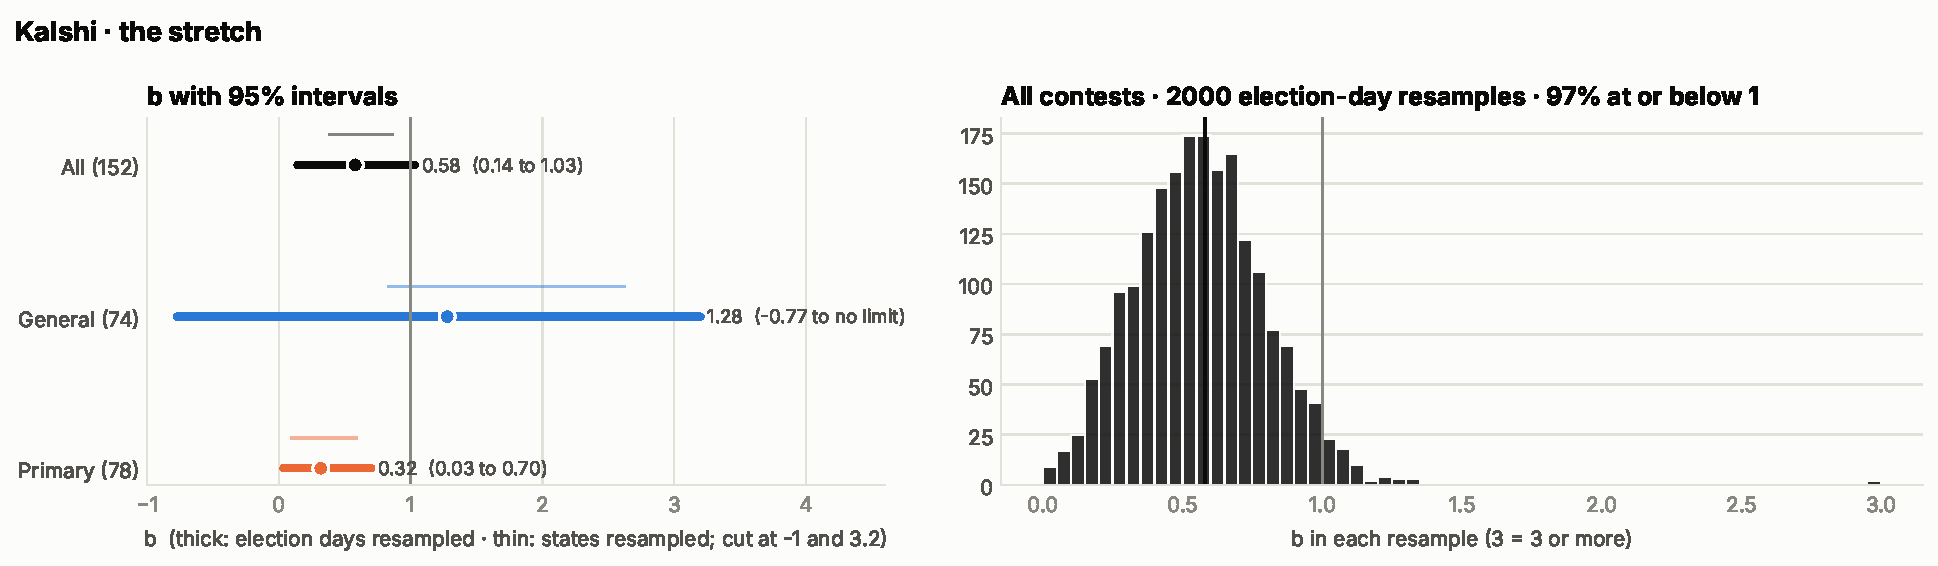
\includegraphics[width=\textwidth]{figures/fit_kalshi_stretch.pdf}\par\medskip
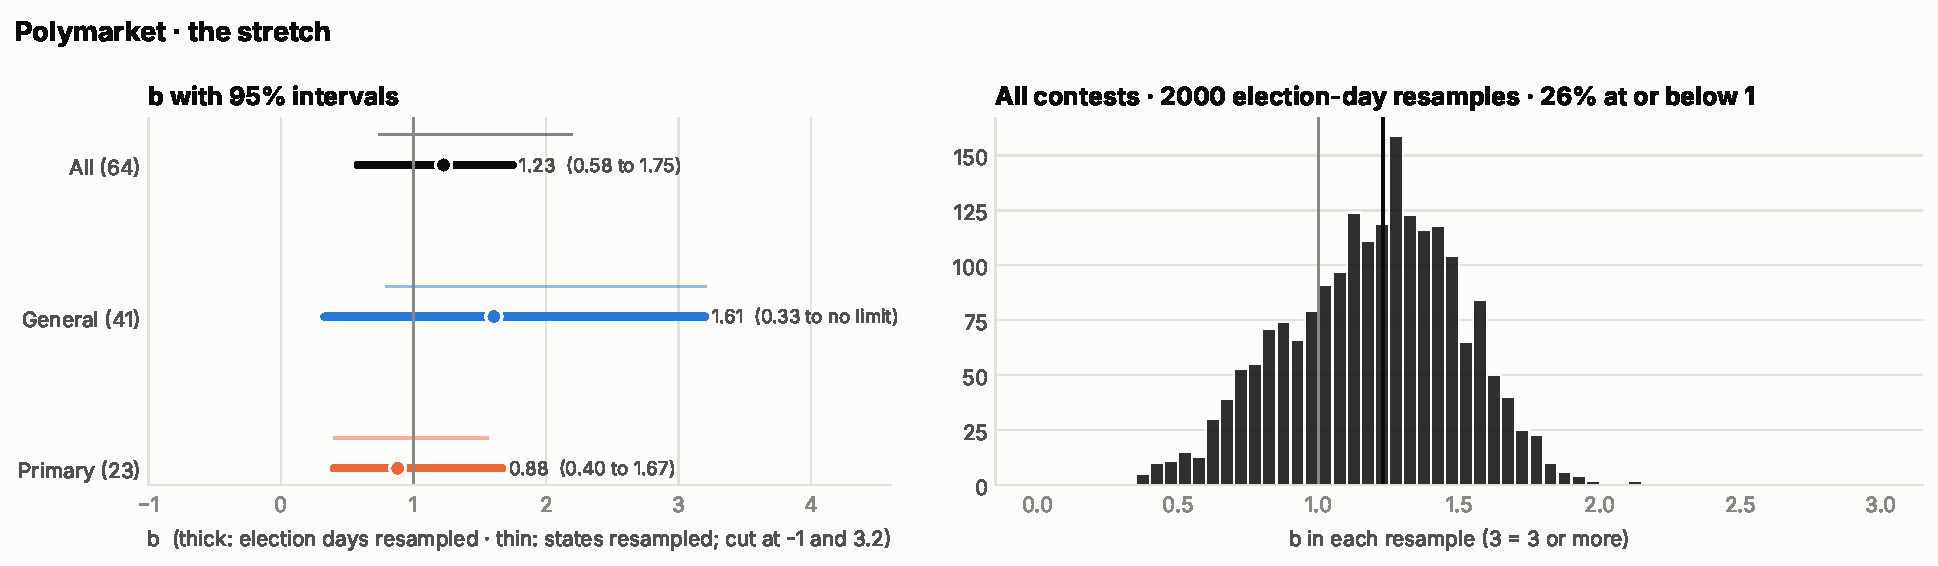
\includegraphics[width=\textwidth]{figures/fit_polymarket_stretch.pdf}
\caption{The stretch in the training period. Left: each group with its interval from resampling election days (thick)
and states (thin). Right: the stretch for all contests, refitted on each of 2,000 resamples of election
days.}\label{fig:train_stretch}
\end{figure}

\paragraph{Robustness.}
No single primary day drives the results (Figure~\ref{fig:lodo}). Leaving out any one election day other than
5 November 2024 keeps Kalshi's overall stretch between 0.53 and 0.69, and Polymarket's between 1.21 and 1.38. Leaving
out 5 November 2024, the night that carries the general-election underconfidence, pulls them down to 0.36 and 0.91.
The same figure shows what happens when one stretch is used for everything. Fitted on all other days and applied to the day left
out, a single stretch barely improves Kalshi's forecasts (log loss 0.001 lower over all contests, better on 14 of 26
days) and worsens Polymarket's (0.025 higher, despite helping on 16 of 23 days). This is what one would expect if the
correction points one way in general elections and the other way in primaries. Adding the contests from other
countries changes little on Kalshi and pulls Polymarket's general-election stretch from 1.61 to 1.15
(Figure~\ref{fig:us_all}). Dropping the five Kalshi contests in which neither candidate traded in the day before the
snapshot gives 0.60, 1.27 and 0.33 for all contests, general elections and primaries.

Kalshi's primary result is also not explained by runoffs (Figure~\ref{fig:primary_checks}). Several upsets were in
states where a primary can go to a runoff, so a market priced on the first round's election day might settle only weeks
later. But outside those states, favourites still lost 16 times where the prices implied 7 (stretch 0.40, 0.03 to
0.83), and 74 of the 78 markets settled within two weeks of the vote (0.33, $-0.01$ to 0.72). In the runoff states the
overconfidence is stronger still: 15 upsets where the prices implied 7 (0.16, $-0.19$ to 1.10). These intervals refit
the stretch with the corrected routine mentioned under Table~\ref{tab:training}.

\begin{figure}[tbp]
\centering
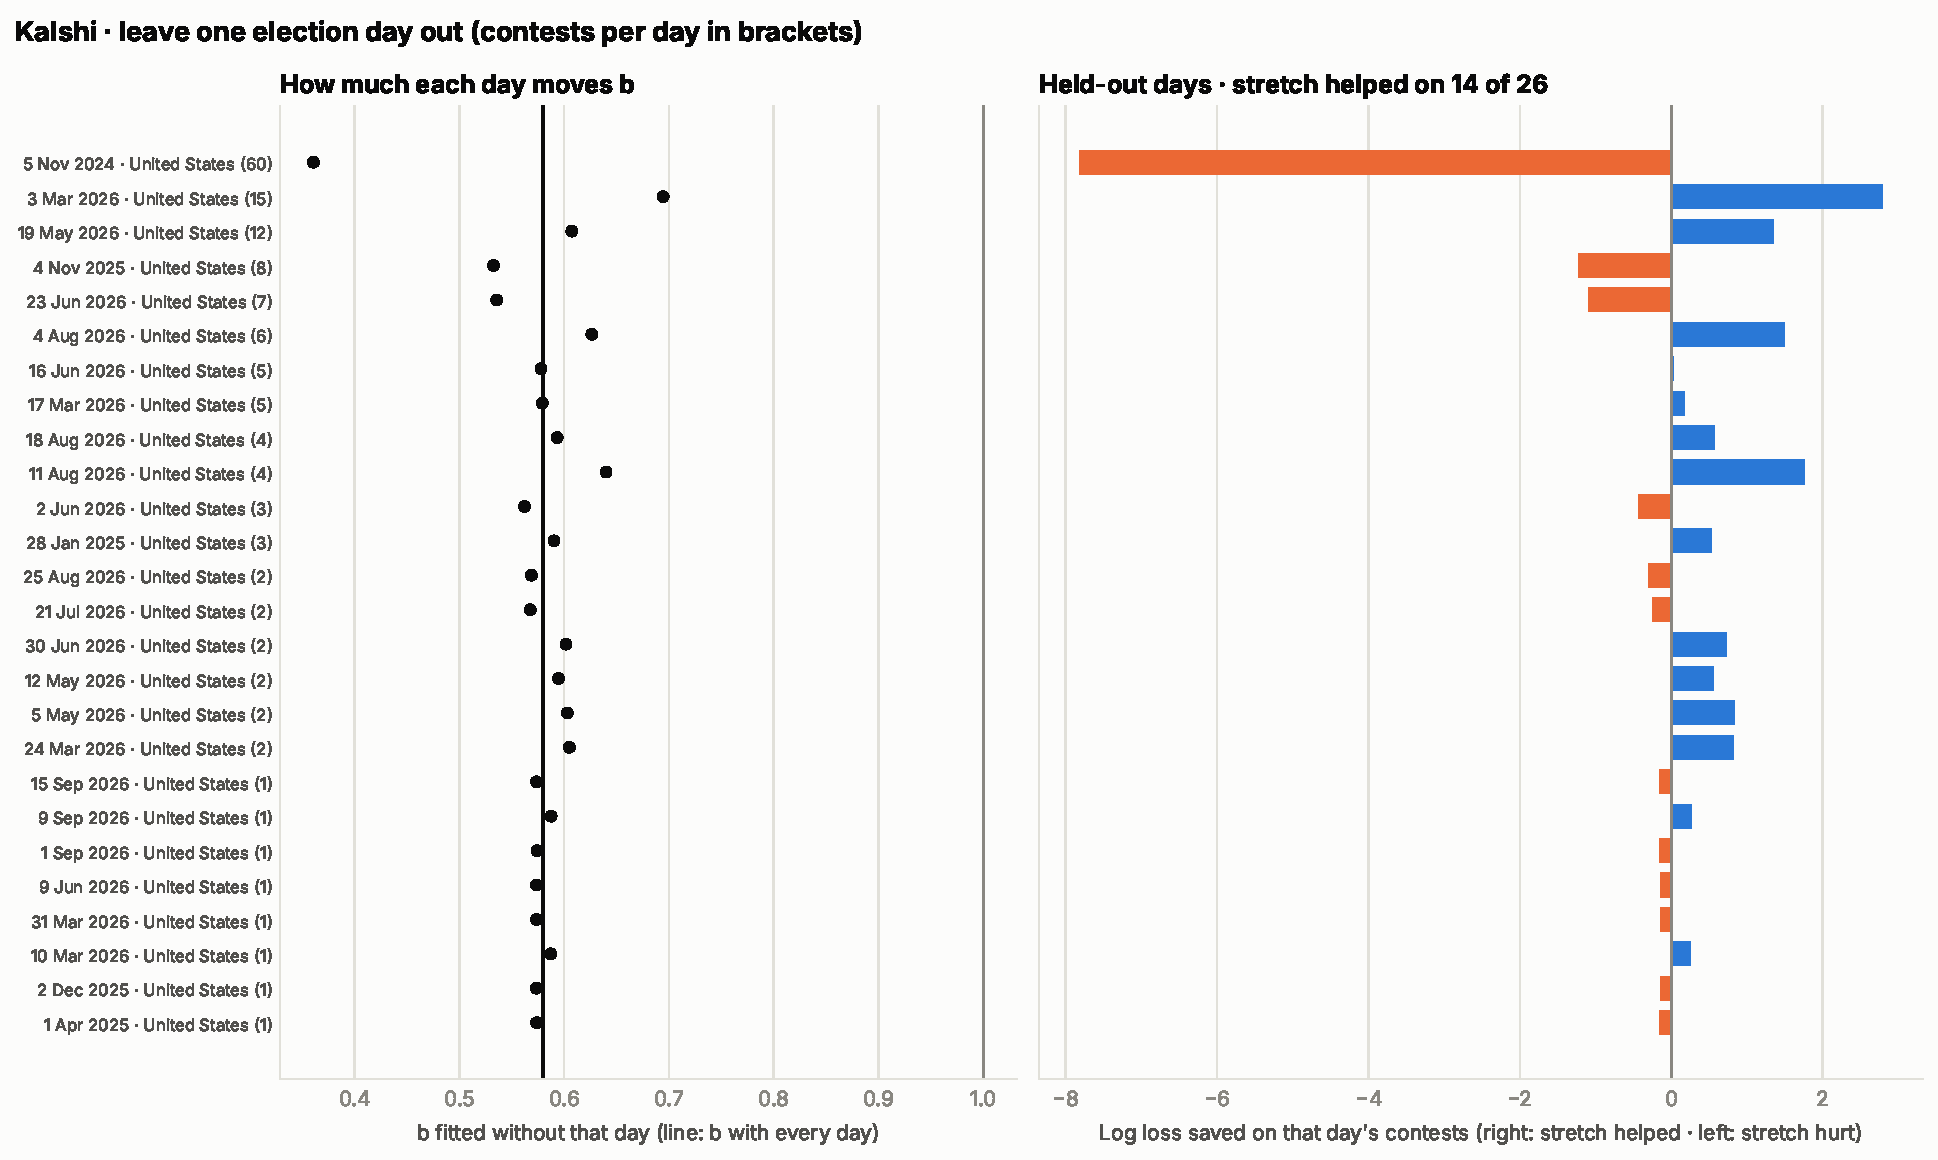
\includegraphics[width=0.92\textwidth]{figures/fit_kalshi_leave_one_day_out.pdf}\par\medskip
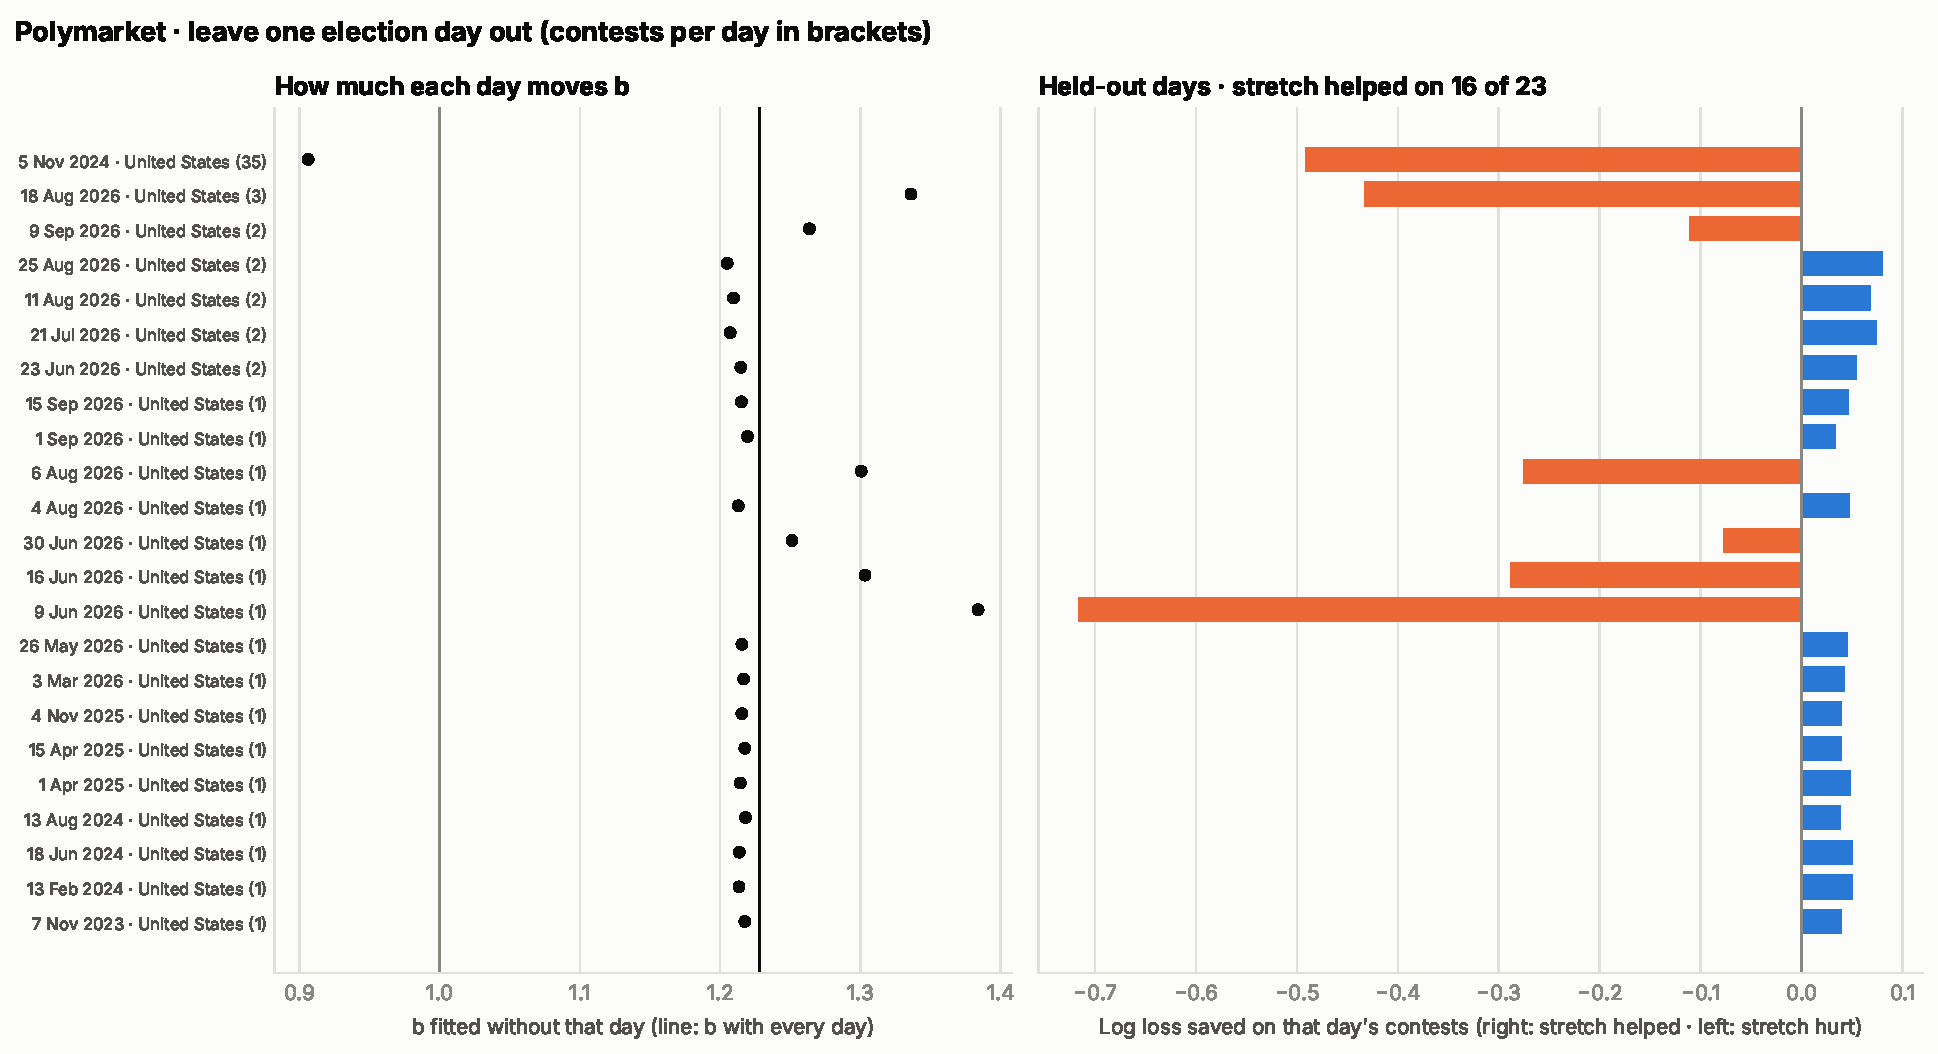
\includegraphics[width=0.92\textwidth]{figures/fit_polymarket_leave_one_day_out.pdf}
\caption{Leaving out one election day at a time. Left: the stretch fitted without that day; the line is the stretch with
every day. Right: how much a stretch fitted on all other days improved (blue) or worsened (orange) the log loss of that
day's contests.}\label{fig:lodo}
\end{figure}

\begin{figure}[tbp]
\centering
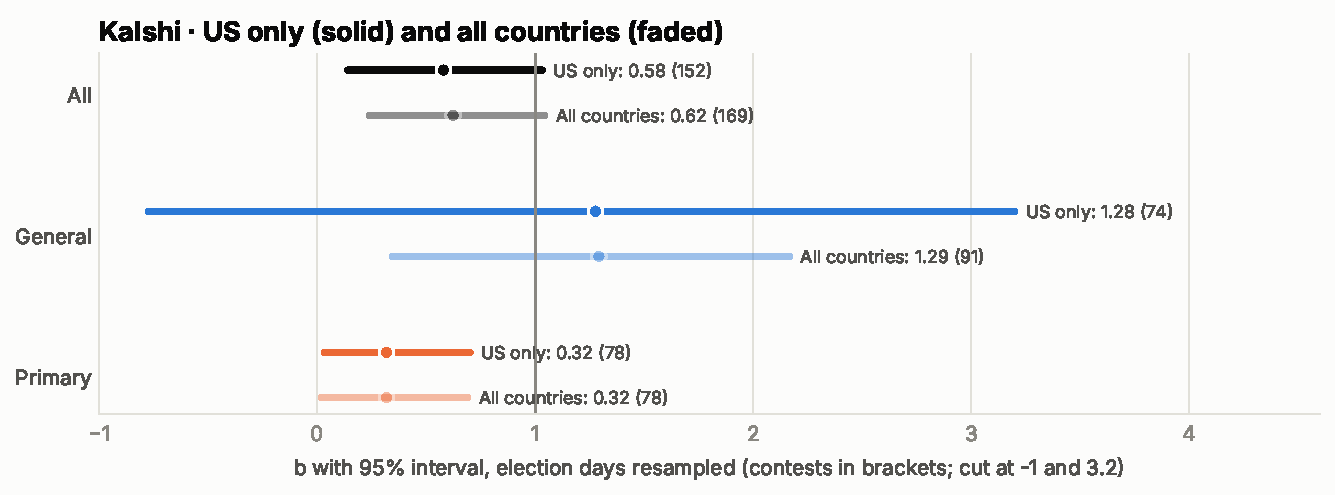
\includegraphics[width=0.85\textwidth]{figures/fit_kalshi_us_vs_all.pdf}\par\medskip
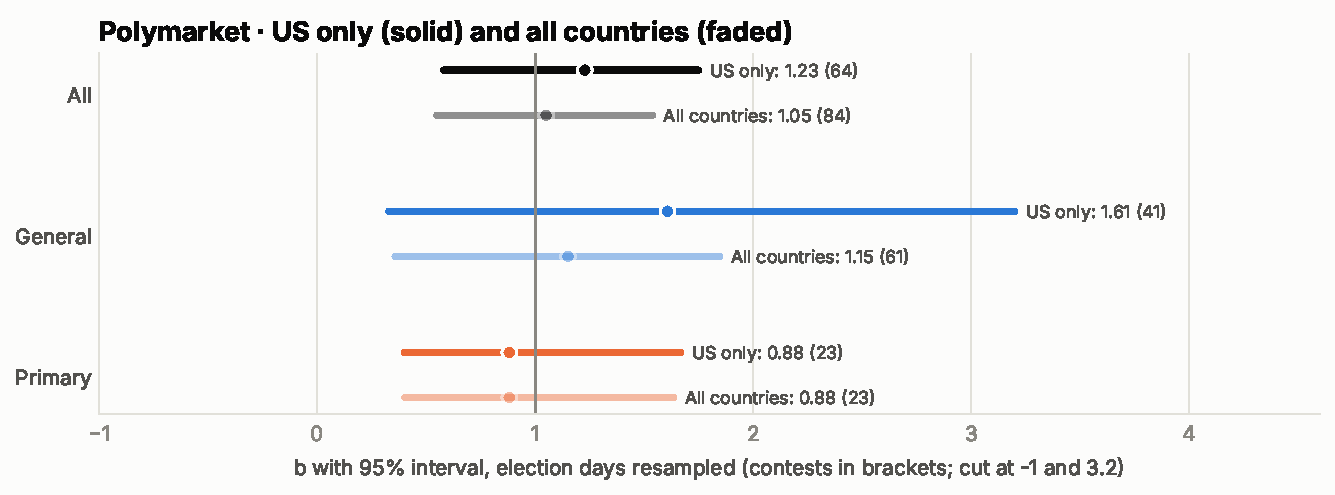
\includegraphics[width=0.85\textwidth]{figures/fit_polymarket_us_vs_all.pdf}
\caption{US contests only (solid) against contests in every country (faded), with intervals from resampling election
days.}\label{fig:us_all}
\end{figure}

\begin{figure}[tbp]
\centering
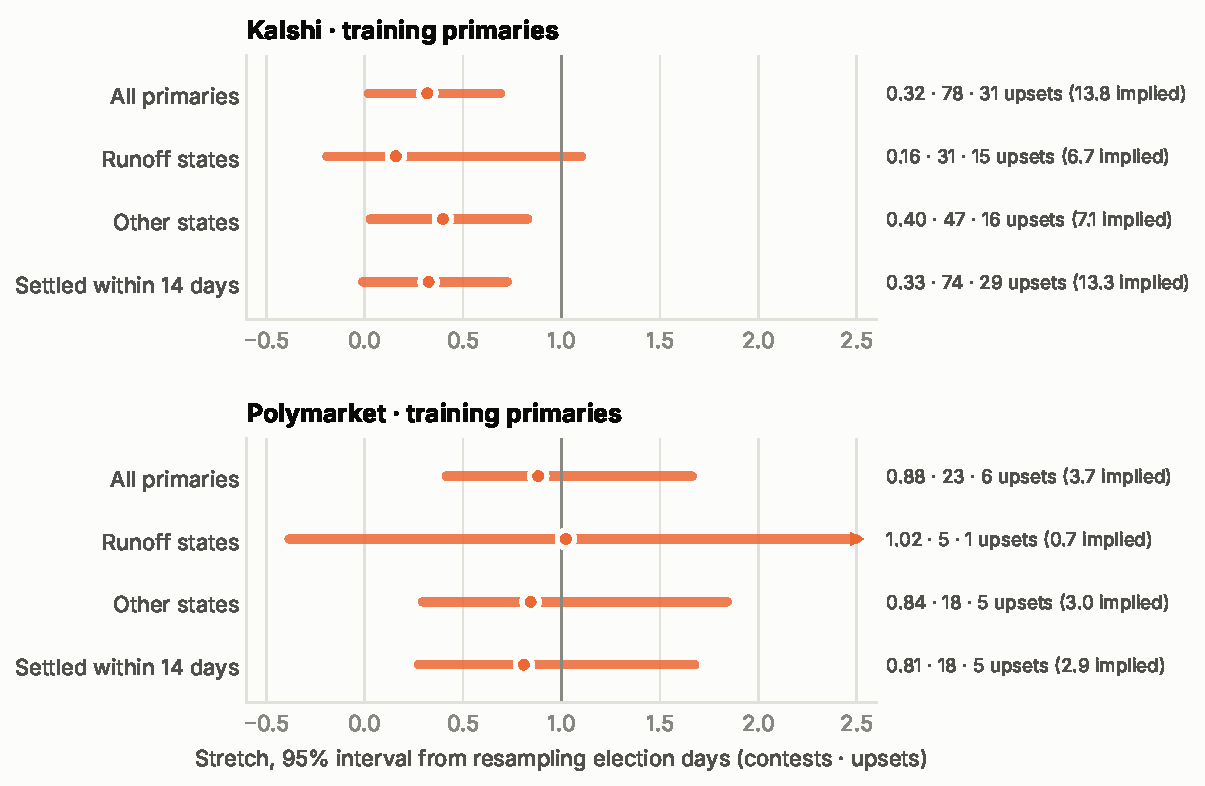
\includegraphics[width=0.85\textwidth]{figures/res_primary_checks.pdf}
\caption{Checks on the training primaries: states where a primary can go to a runoff, other states, and markets that
settled within 14 days of the vote. Intervals resample the primaries' election days, refitting with the corrected
routine, so the first row differs slightly from Table~\ref{tab:training}; arrows mark intervals that run past the edge.
Labels give the stretch, the number of contests, and the upsets against the number the prices
implied.}\label{fig:primary_checks}
\end{figure}

\subsection{The pre-registered midterm test}

Table~\ref{tab:test} reports the preliminary run of the test, on the contests settled by 10 November 2026.
On Polymarket, the stretch of the 145 midterm contests was 1.66, with an interval from 1.21 to 2.91. The whole interval
lies above 1, so Polymarket's general-election markets were \emph{underconfident}, and it includes the 2024 value of
1.83, so they were \emph{consistent with 2024}. The pre-registered reading is that underconfidence persists in general
elections, which supports the explanation that primaries are traded differently. On Kalshi, the stretch of the 187
contests was 1.32, with an interval from 0.88 to 2.35. It includes 1, so there is no detectable miscalibration, and it
includes the 2024 value of 1.97, so it is also consistent with 2024. The pre-registered reading is \emph{inconclusive}.

\begin{table}[htbp]
\centering\small\setlength{\tabcolsep}{4.5pt}
\caption{The pre-registered midterm test, preliminary run of 10 November 2026. Intervals resample states. Forty listed
contests had not yet settled.}\label{tab:test}
\begin{tabular}{lL{1.5cm}L{2.1cm}L{2.5cm}L{2.4cm}L{3.1cm}}
\toprule
 & Contests (states) & Stretch (95\% interval) & Level & Change & Reading \\
\midrule
Kalshi & 187 (36) & 1.32\newline (0.88 to 2.35) & No detectable miscalibration & Consistent with 2024 (1.97) & Inconclusive \\
\addlinespace
Polymarket & 145 (34) & 1.66\newline (1.21 to 2.91) & Underconfident & Consistent with 2024 (1.83) & Underconfidence persists in general elections \\
\bottomrule
\end{tabular}
\end{table}

Figure~\ref{fig:test} draws the test itself. Each panel is the distribution of the stretch over the 2,000 resamples of
states, the same resamples the test used. On Polymarket, all but 4 of the 2{,}000 lie above 1. On Kalshi, 92\% do,
short of the 97.5\% that an interval wholly above 1 requires. Figure~\ref{fig:cmp_stretch} places the midterm values next to every training
group. On both platforms the midterms sit with the earlier general elections and far from the earlier primaries.

\begin{figure}[tbp]
\centering
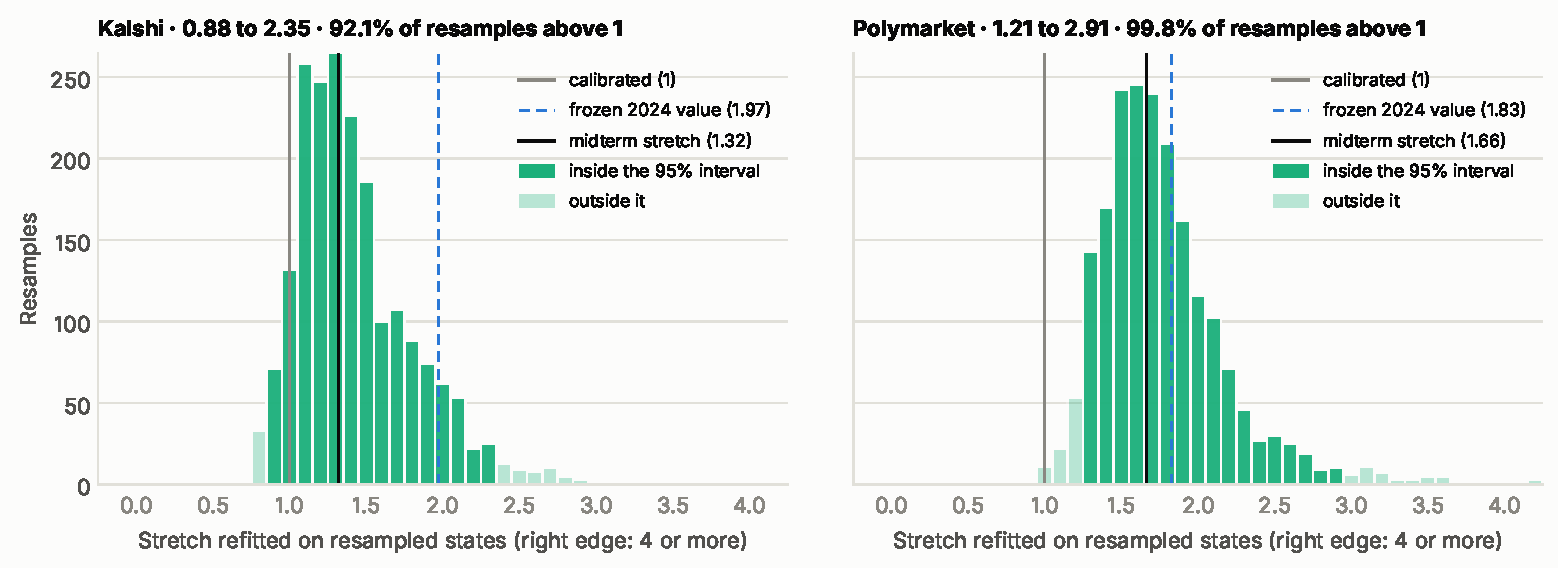
\includegraphics[width=\textwidth]{figures/res_test_resamples.pdf}
\caption{The pre-registered test. The stretch refitted on each of 2,000 resamples of states; the darker bars are the
central 95\%, which is the test's interval. Grey: a calibrated market. Dashed blue: the frozen 2024 value. Black: the
midterm stretch.}\label{fig:test}
\end{figure}

\begin{figure}[tbp]
\centering
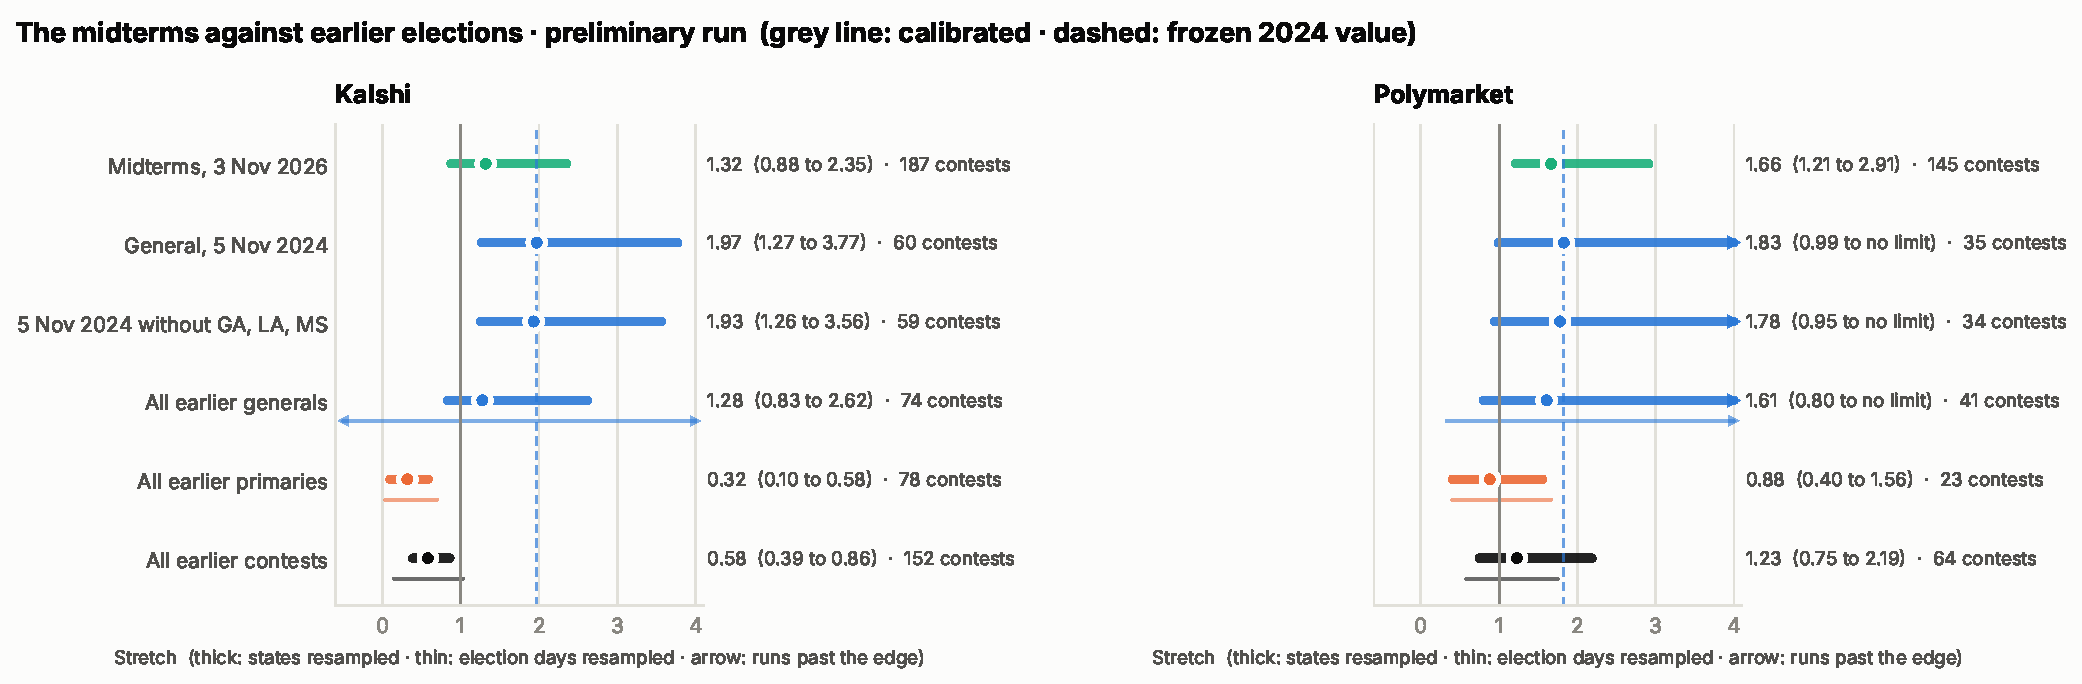
\includegraphics[width=\textwidth]{figures/cmp_stretch.pdf}
\caption{The midterms against the training groups. Thick bars resample states; thin bars, for groups spanning several
election days, resample days. Grey line: a calibrated market. Dashed line: the frozen 2024 value.}\label{fig:cmp_stretch}
\end{figure}

\subsection{Exploratory analyses}\label{sec:exploratory}

Everything in this subsection was examined after the vote. The p-values reported here are descriptive, and several
comparisons were made, so a single result near the 5\% level should be read with caution.

\paragraph{Favourites priced above 80\% almost never lost.}
Figure~\ref{fig:cmp_calibration} compares the midterms with the 2024 night and the earlier primaries, price group by
price group. Midterm favourites priced between 80\% and 95\% won 99 of 104 contests on Kalshi and 83 of 84 on
Polymarket, against average prices of about 85\% to 93\%. Close races were priced about right or slightly too
confidently: favourites priced between 50\% and 70\% won 52\% of the time on Kalshi and 58\% on Polymarket, against an
average price of about 60\%. The underconfidence therefore sits in clear favourites, not in tossups. In all, prices
implied 39 upsets on Kalshi and 29 on Polymarket; there were 35 and 20.

\begin{figure}[tbp]
\centering
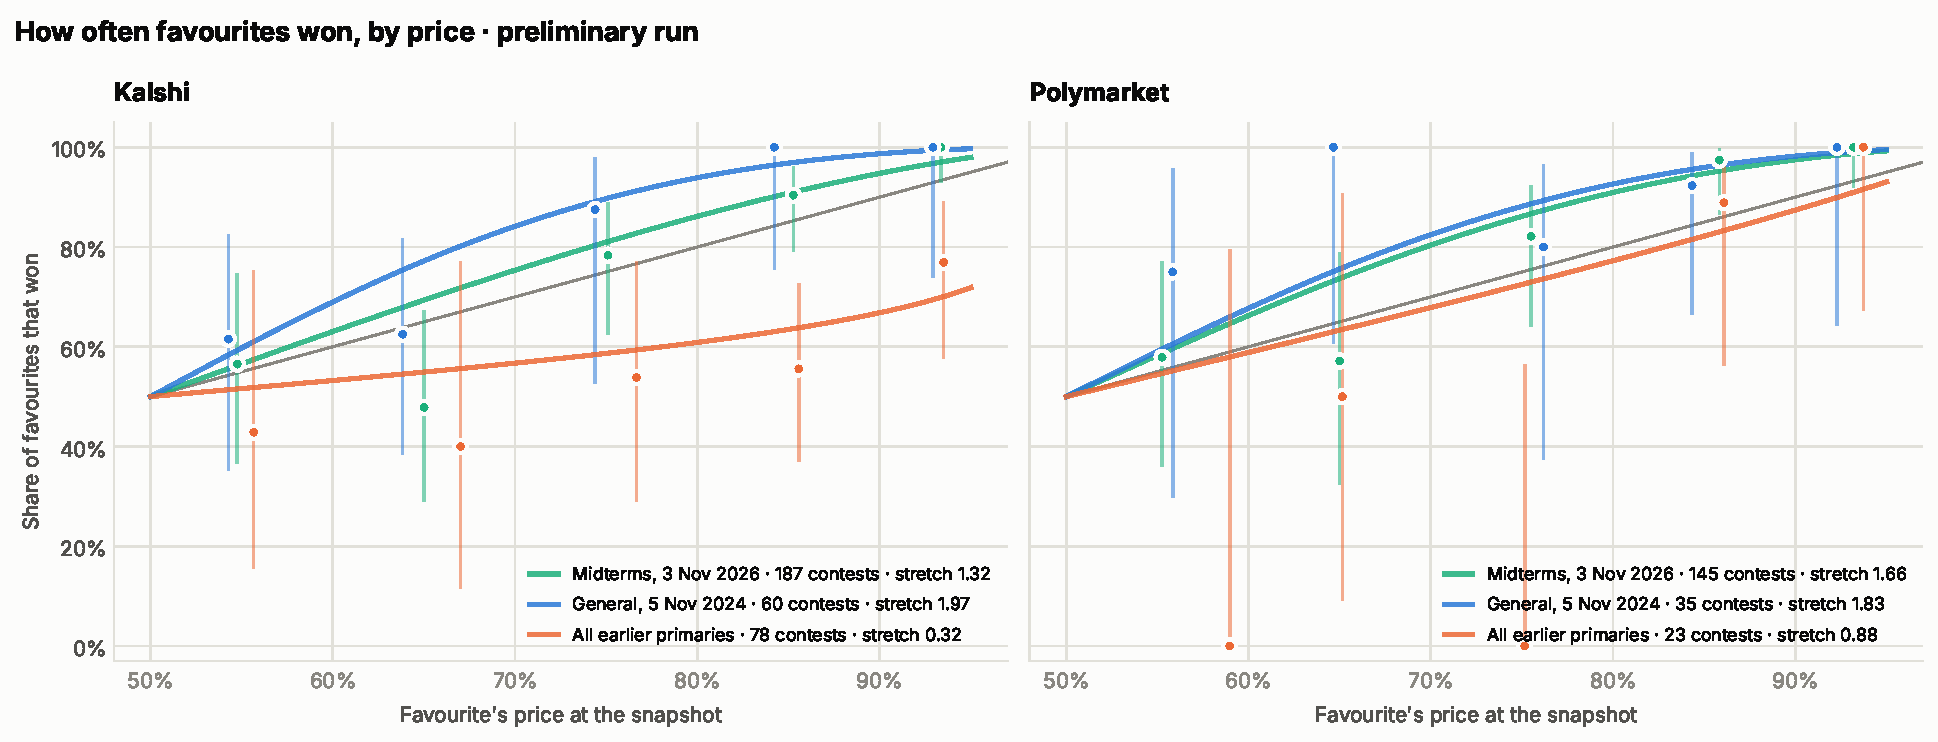
\includegraphics[width=\textwidth]{figures/cmp_calibration.pdf}
\caption{How often favourites won, by price: the midterms (green), the 2024 night (blue) and the training primaries
(orange). Dots: share of favourites that won in each price group, with 95\% intervals. Lines: each group's fitted
stretch. Grey diagonal: a calibrated market.}\label{fig:cmp_calibration}
\end{figure}

\paragraph{Every general-election night looks alike.}
Figure~\ref{fig:cmp_days} shows each election day with at least five contests: how many points more often favourites
won than their average price implied. On the midterms, the gap was $+2.0$ points on Kalshi and $+6.1$ on Polymarket.
On 5 November 2024 it was $+6.8$ and $+12.7$, and on Kalshi's eight contests of 4 November 2025, every favourite won, a gap of
$+13.7$. Of the six Kalshi days that include primaries, four lie below zero, two of them by more than 40 points;
Polymarket has no primary day with five contests.

\begin{figure}[tbp]
\centering
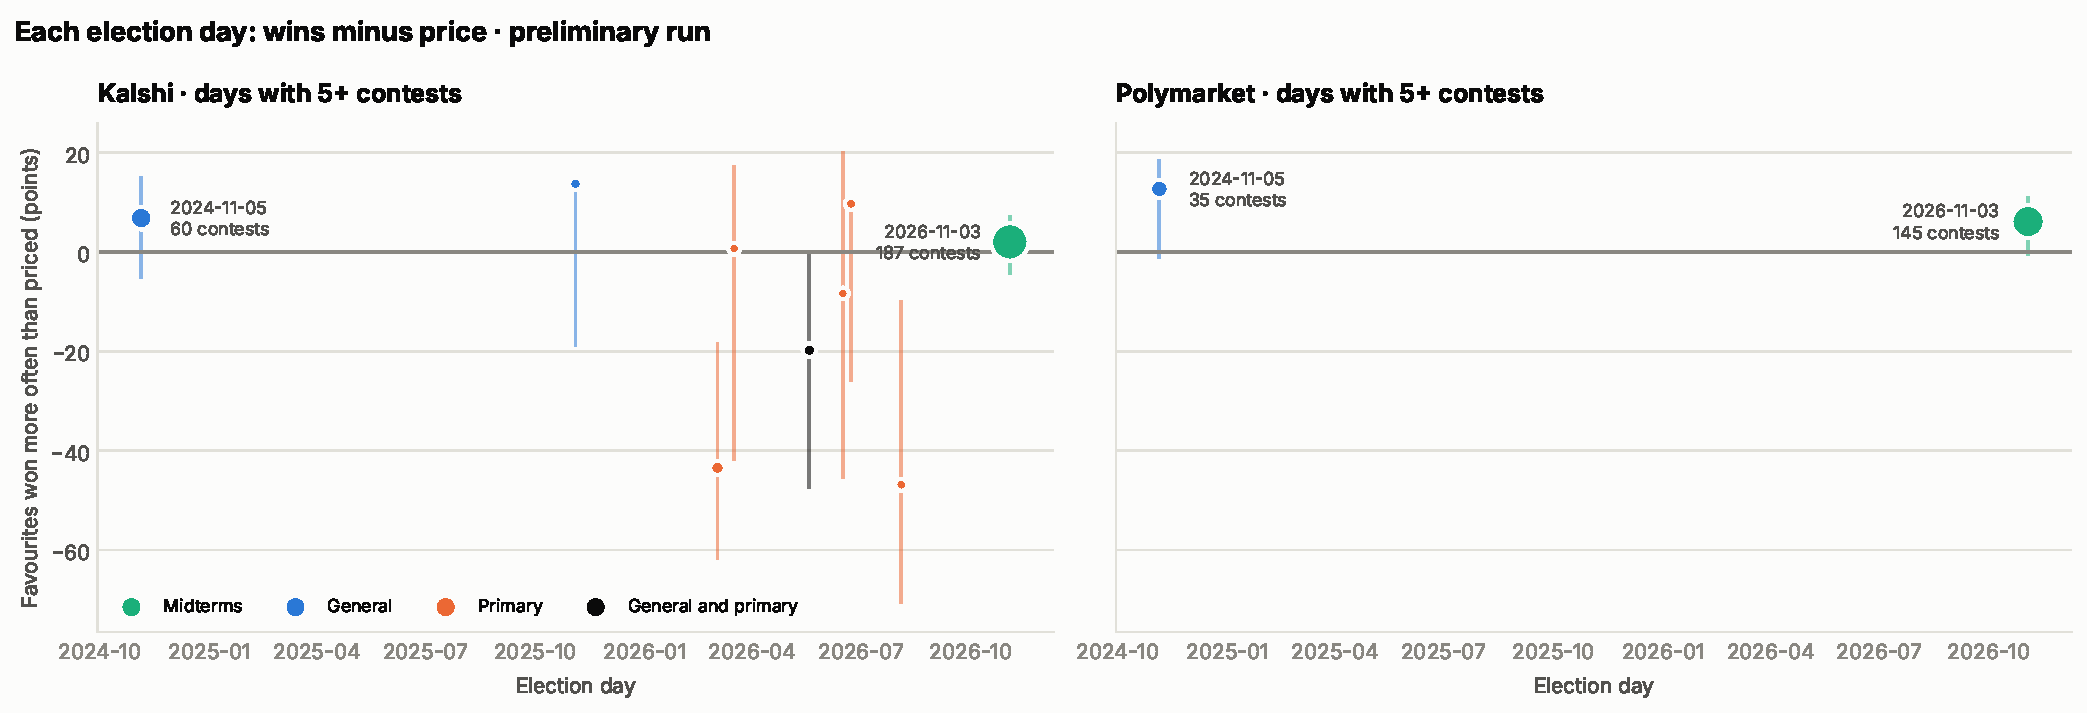
\includegraphics[width=\textwidth]{figures/cmp_election_days.pdf}
\caption{Each election day with at least five contests: share of favourites that won minus their average price, in
percentage points, with a 95\% interval. Dot size: number of contests. Above zero, favourites won more often than
priced.}\label{fig:cmp_days}
\end{figure}

\paragraph{Upsets cluster by state.}
Figure~\ref{fig:upsets} shows where the midterm upsets fell. On Kalshi, Texas alone had 12 upsets where the prices
implied 5, and North Carolina 4 where they implied 1.5; Florida had 1 where they implied 4.2. Polymarket shows the same
places, more mildly. This clustering is why every interval resamples whole states: the 187 Kalshi contests carry closer
to 36 states' worth of independent information than to 187 contests' worth.

\begin{figure}[tbp]
\centering
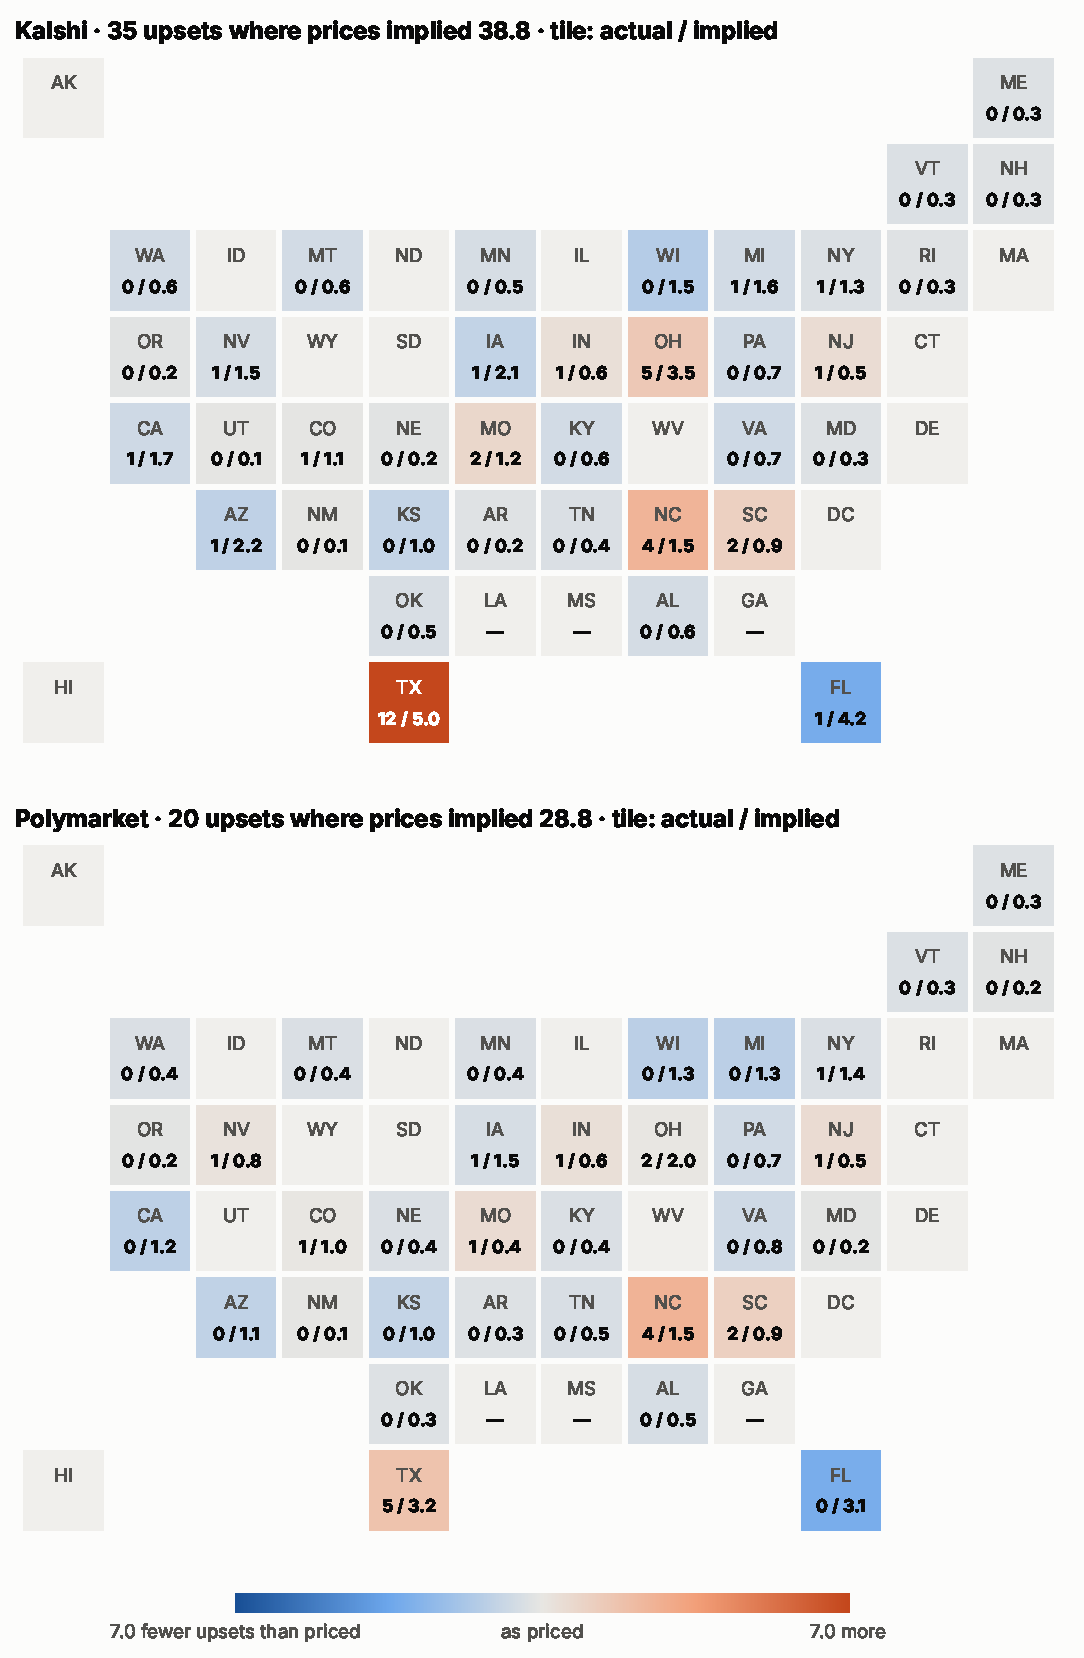
\includegraphics[width=0.74\textwidth]{figures/res_upsets_map.pdf}
\caption{Midterm upsets by state: the number of favourites that lost, against the number the prices implied (the sum of
one minus the favourite's price). Blue: fewer upsets than priced. Orange: more. Georgia, Louisiana and Mississippi were
excluded in advance.}\label{fig:upsets}
\end{figure}

\paragraph{On the same races, the two platforms agree.}
Kalshi's weaker result does not come from pricing races differently. On the 141 races that both platforms listed and
that passed every rule on both, the two had the same favourite every time, and their chances for the eventual winner
differed by 0.9 percentage points on average (Figure~\ref{fig:same_scatter}). On these shared races, both platforms were
underconfident: 1.68 on Kalshi (1.21 to 3.00) and 1.65 on Polymarket (1.18 to 2.89), with 20 upsets each where the
prices implied about 29 (Figure~\ref{fig:same_split}). The difference lies in the 46 races that only Kalshi listed: mostly down-ballot statewide offices such as
treasurer and attorney general, eight state supreme court seats, three mayors and three state legislative seats, with
nine House seats. There, favourites lost 15 times where the prices implied 10, a stretch of 0.75 (0.38 to 2.04). Six of
the 15 upsets were supreme court seats in Texas and Ohio. Resampling states jointly, Kalshi's overall stretch minus Polymarket's is $-0.34$, with
an interval from $-0.79$ to $0.09$: Kalshi came out lower in 91\% of resamples, but the difference is not significant.
The training data show a similar pattern on a much smaller scale. Kalshi's 14 general-election contests outside the
2024 night had 4 upsets where the prices implied 2, all in low-profile 2026 races: two Florida legislative special
elections and two Georgia Supreme Court seats. If the prices had been right, four or more upsets would have occurred
14\% of the time.

\begin{figure}[tbp]
\centering
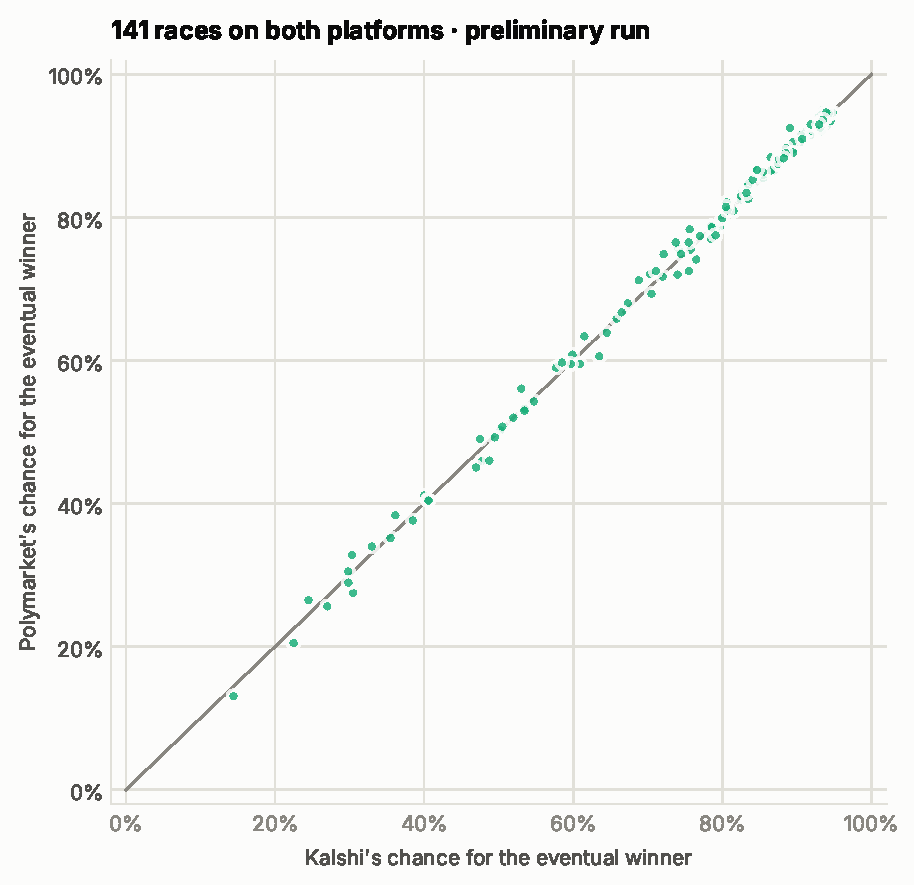
\includegraphics[width=0.5\textwidth]{figures/cmp_same_races.pdf}
\caption{The 141 midterm races on both platforms: the chance each gave the candidate who won. Dots above the diagonal
mean Polymarket gave the winner more.}\label{fig:same_scatter}
\end{figure}

\begin{figure}[tbp]
\centering
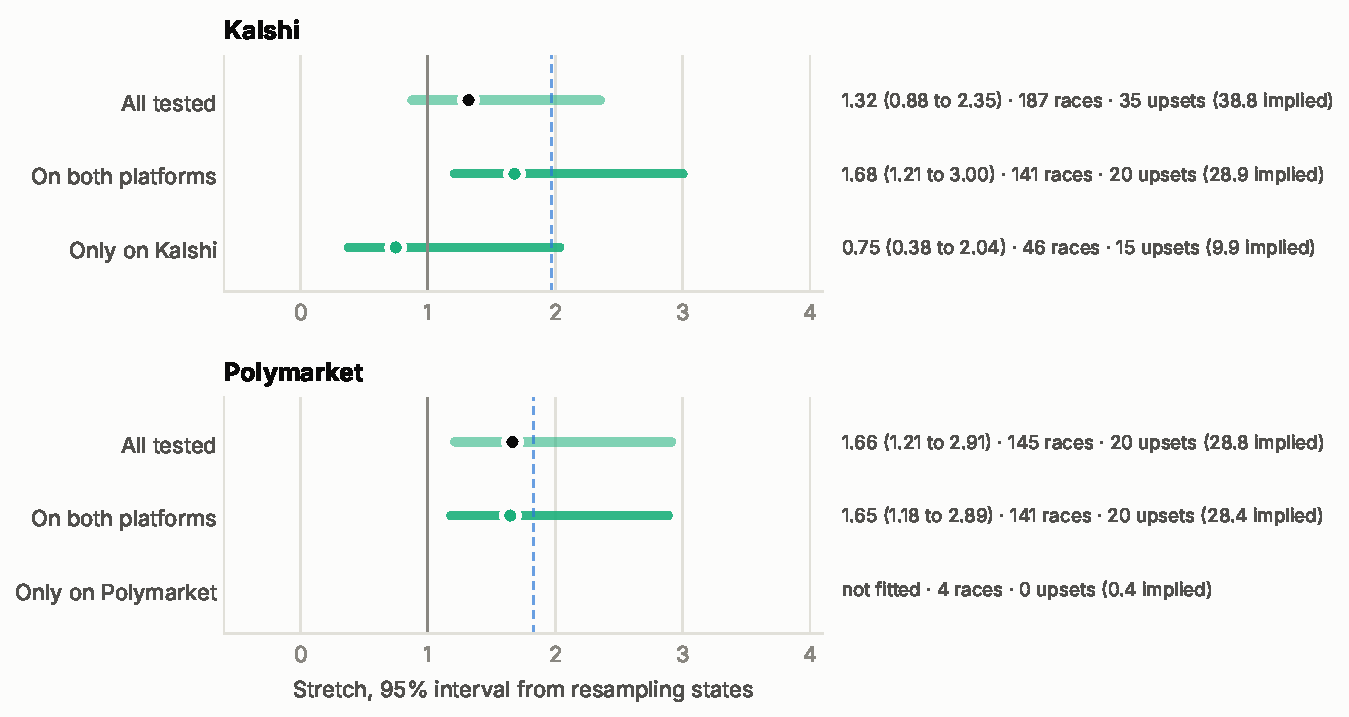
\includegraphics[width=0.92\textwidth]{figures/res_same_races.pdf}
\caption{Each platform's midterm contests split into races on both platforms and races on that platform only.
Intervals resample states. Grey line: a calibrated market. Dashed line: the frozen 2024 value. Polymarket listed only
four races that Kalshi did not, too few to fit.}\label{fig:same_split}
\end{figure}

\paragraph{Would the earlier stretch have improved the midterm prices?}
Applying a stretch fixed before the vote to the midterm prices tests the correction out of sample
(Figure~\ref{fig:scores}). On Polymarket, every value learned from general elections improved the log loss by close to
the most any single stretch could have: the frozen 2024 value by 0.032 ($-0.027$ to 0.081), the value from all earlier
general elections by 0.033 ($-0.010$ to 0.069), against a ceiling of 0.033. On Kalshi, the earlier general-election
value improved it slightly (0.010, $-0.020$ to 0.036, equal to the ceiling), while the 2024 value overcorrected and
made it slightly worse ($-0.017$). Values learned from primaries made the prices clearly worse on both platforms: by
0.143 on Kalshi and 0.016 on Polymarket, with intervals that exclude zero. A correction learned from general elections
carries over to the next general election; one learned from primaries does not.

\begin{figure}[tbp]
\centering
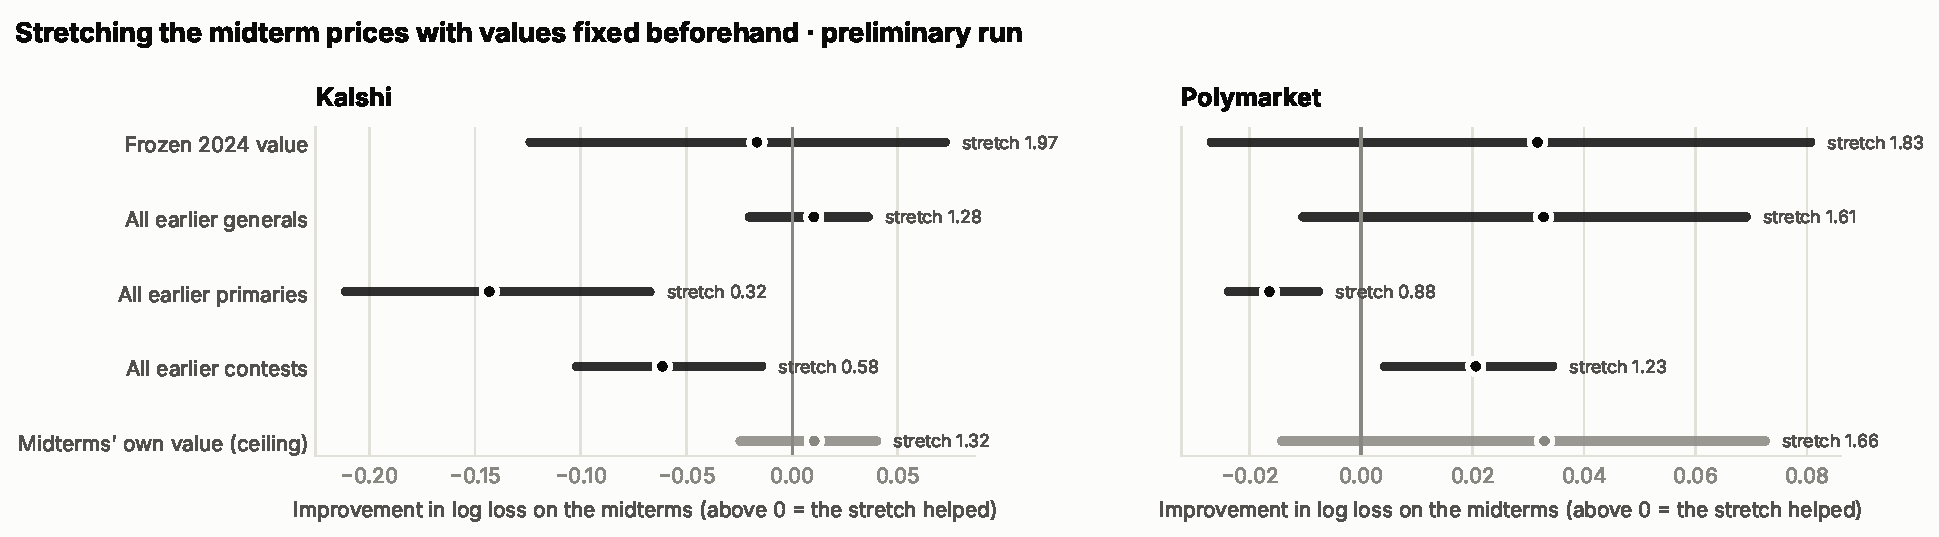
\includegraphics[width=\textwidth]{figures/cmp_scores.pdf}
\caption{Improvement in the log loss of the midterm prices when each is stretched by a value fixed before the vote.
Above zero, the stretch helped. Intervals resample states with the stretch held fixed. The last row uses the midterms'
own stretch and marks the best any single value could have done.}\label{fig:scores}
\end{figure}

\paragraph{How strong is the evidence?}
Table~\ref{tab:pvalues} gives p-values for the two questions, computed naively and allowing for contests in one state
moving together (the column headed ``$p$, states''). Allowing for states matters a great deal. On Polymarket, the midterm stretch is clearly above 1 either
way ($p = 0.02$ allowing for states; 0.2\% of state resamples at or below 1). On Kalshi it is not ($p = 0.15$).
Persistence is weaker. Stretching Polymarket's midterm prices by the 2024 value made the results about 99 times as
likely as the raw prices did, which looks decisive if contests are treated as independent, but gives $p = 0.13$ once
states are allowed to move together. With the value from all earlier general elections, $p = 0.06$. A single election
night of about 35 states cannot establish persistence on its own.

\begin{table}[tbp]
\centering\small
\caption{Exploratory p-values, one-sided. Level: is the midterm stretch above 1? Persistence: does a stretch fixed
before the vote make the midterm results more likely than the raw prices do? ``Times as likely'' is the ratio of the
two likelihoods. ``${\le}\,1$'' is the share of the test's state resamples at or below 1. ``$p$, states'' allows for contests
in one state moving together.}\label{tab:pvalues}
\setlength{\tabcolsep}{4.5pt}
\begin{tabular}{llrrrr}
\toprule
 & Question & ${\le}\,1$ & Times as likely & Naive $p$ & $p$, states \\
\midrule
Kalshi & Level & 7.9\% & & 0.024 & 0.153 \\
 & Persistence, 2024 value (1.97) & & 0.04 & 0.750 & 0.622 \\
 & Persistence, earlier generals (1.28) & & 6.8 & 0.073 & 0.235 \\
\midrule
Polymarket & Level & 0.2\% & & 0.001 & 0.022 \\
 & Persistence, 2024 value (1.83) & & 98.6 & 0.044 & 0.133 \\
 & Persistence, earlier generals (1.61) & & 115.5 & 0.008 & 0.062 \\
\bottomrule
\end{tabular}
\end{table}

\subsection{Summary}

General-election markets on both platforms were underconfident in 2024 and, on the races both platforms listed,
equally underconfident in the 2026 midterms. Polymarket passed the pre-registered test; Kalshi's result is inconclusive,
because the low-profile races only Kalshi listed went the other way. Kalshi's primaries were strongly overconfident in
the training data, a result not explained by runoffs or late settlement, and corrections learned from primaries made
midterm prices worse. The pattern is consistent with primaries being traded differently from general elections, and
not with the underconfidence having faded over time.
